\section{Спектральное дифференцирование на промежутке \mbox{[-100, 100]}}\label{app:A}

\subsection{Исходная функция}
Рассмотрим функцию $f(t) = sin(t)$ и соответствующий ей массив точек на промежутке $[-100, 100]$ с 
наложенным на нее небольшой случайный шум. График полученный функции приведен на рисунке \ref{fig:noised_sin_100}.

\begin{figure}[ht!]
    \centering
    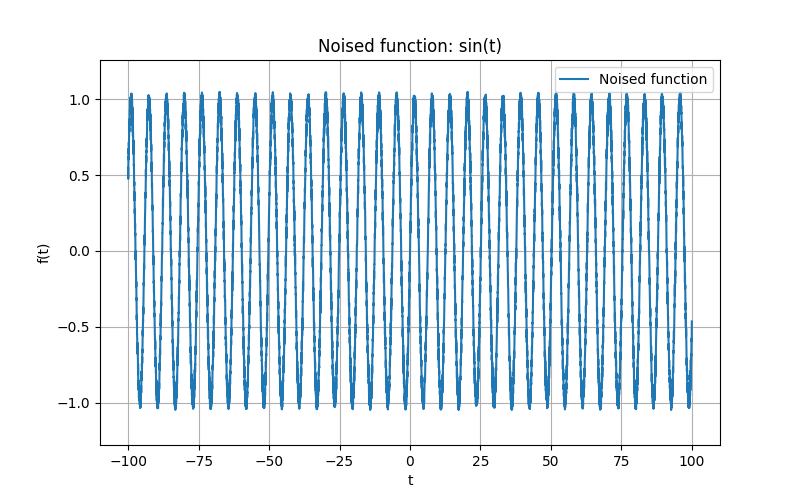
\includegraphics[width=\textwidth]{../results/100/noised_sin.png}
    \caption{Функция $f(t) = sin(t)$ с небольшим случайным шумом}
    \label{fig:noised_sin_100}
\end{figure}

\FloatBarrier
\subsection{Численная производная}
График численной производной приведен на рисунке \ref{fig:diff_noised_sin_100}.

\begin{figure}[ht!]
    \centering
    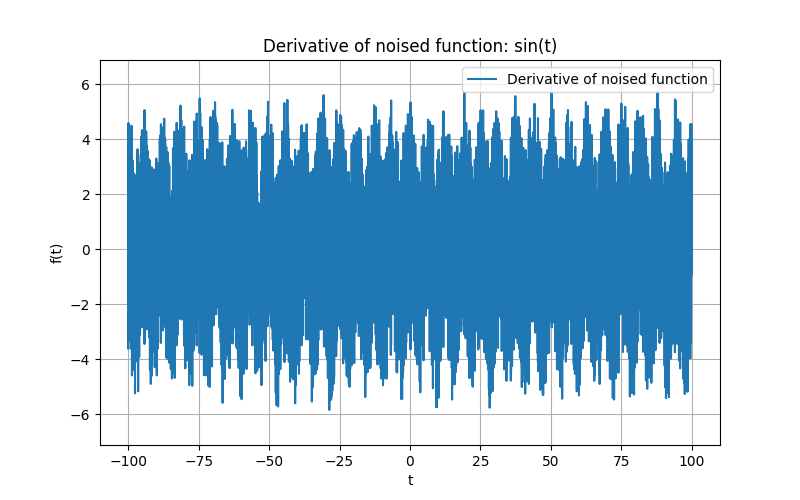
\includegraphics[width=\textwidth]{../results/100/noised_sin_derivative.png}
    \caption{Численная производная функции $f(t) = sin(t)$}
    \label{fig:diff_noised_sin_100}
\end{figure}

\FloatBarrier
\subsection{Спектральная производная}
Для нахождения спектральной производной найдем образ исходной функции $f(t)$ (см. рисунок \ref{fig:noised_sin_image_100}). 
\begin{figure}[ht!]
    \centering
    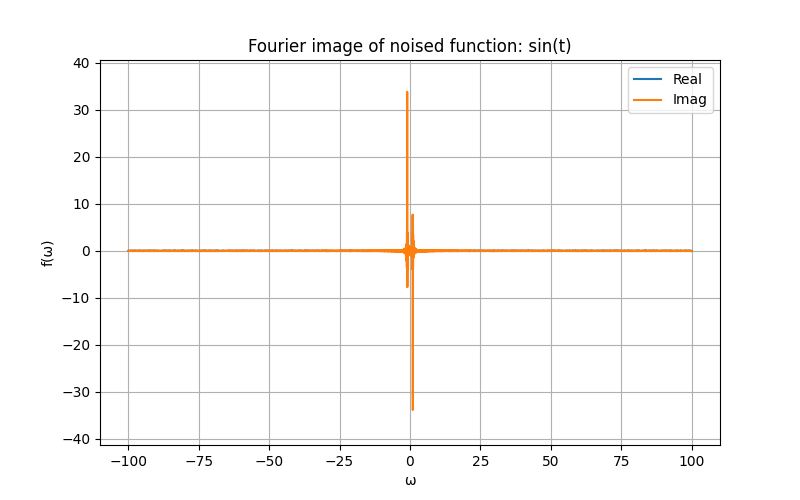
\includegraphics[width=\textwidth]{../results/100/noised_sin_image.png}
    \caption{Образ функции $f(t) = sin(t)$}
    \label{fig:noised_sin_image_100}
\end{figure}
Спектральная производная приведена на рисунке \ref{fig:noised_sin_image_deriviate_100}.

\begin{figure}[ht!]
    \centering
    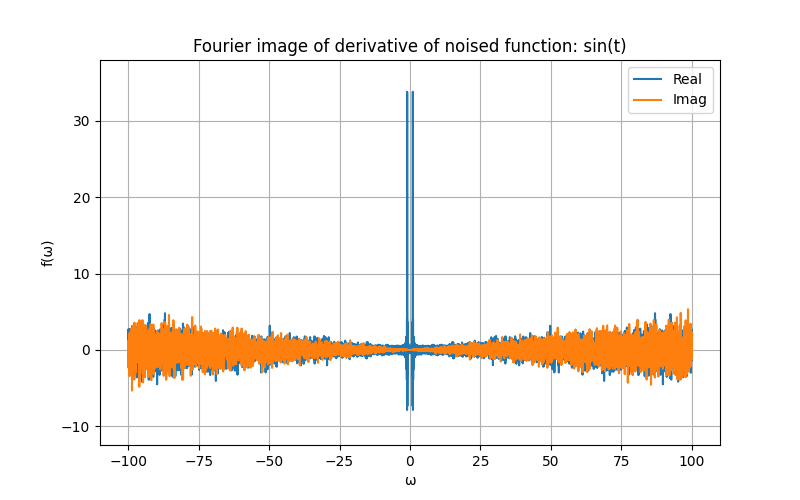
\includegraphics[width=\textwidth]{../results/100/noised_sin_image_derivative.png}
    \caption{Образ производной функции $f(t) = sin(t)$}
    \label{fig:noised_sin_image_deriviate_100}
\end{figure}
Найдем обратное преобразование Фурье от образа производной функции (см. рисунок \ref{fig:noised_sin_image_deriviate_restored_100}) и сравним его с численной производной и истиной производной $(cos(t))$ (см. рисунок \ref{fig:derivative_cmp_100}).

\begin{figure}[ht!]
    \centering
    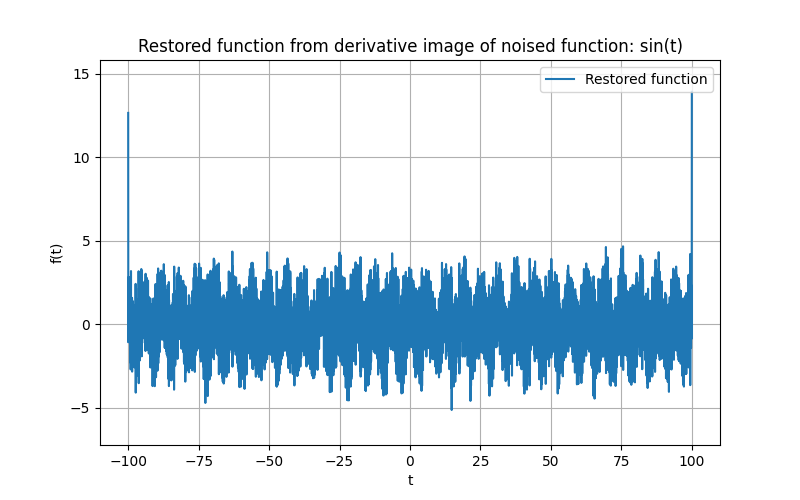
\includegraphics[width=\textwidth]{../results/100/noised_sin_image_derivative_restored.png}
    \caption{Обратное преобразование Фурье от образа производной функции $f(t) = sin(t)$}
    \label{fig:noised_sin_image_deriviate_restored_100}
\end{figure}

\begin{figure}[ht!]
    \centering
    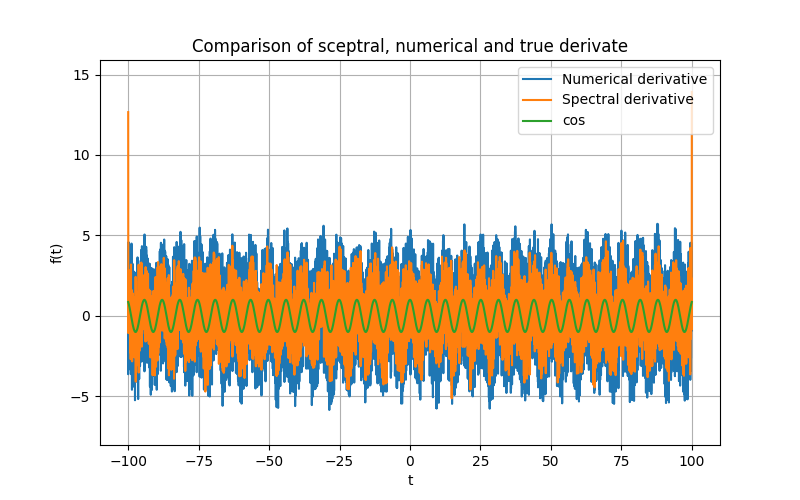
\includegraphics[width=\textwidth]{../results/100/derivative_cmp.png}
    \caption{Сравнение численной производной, истинной производной и спектральной производной}
    \label{fig:derivative_cmp_100}
\end{figure}

\FloatBarrier
На сравнительном графике (см. рисунок \ref{fig:derivative_cmp_100}) видно, что спектральная производная не совпадает с истинной производной функции $f(t) = sin(t)$, в то же время как и численная производная.
В этом случае образ функции обрезан по большему промежутку и включает в себя высокочастотный шум, это можно увидеть на рисунке \ref{fig:noised_sin_image_100}. Это приводит к тому, 
что спектральная производная не совпадает с истинной производной, зато больше совпадает с численной производной. 
